\section{Results}
In figures~\ref{release_bsa_0607} and~\ref{release_bca_0607}, results for the beam-helicity and beam-charge asymmetry amplitudes extracted from the 2006-2007 hydrogen data sets in this work are compared with results extracted in  from the 1996-2005 data set published previously~\cite{Air09}. Each of the asymmetry amplitudes is shown extracted in one bin over all kinematic variables (``overall'') and also projected against $-t$, $x_{\textrm{B}}$ and $Q^{2}$. The beam-helicity asymmetry amplitudes are subject to an additional scale uncertainty from the measurement of the beam polarisation, which is stated in the captions of the figures.
\begin{figure}
\begin{center}
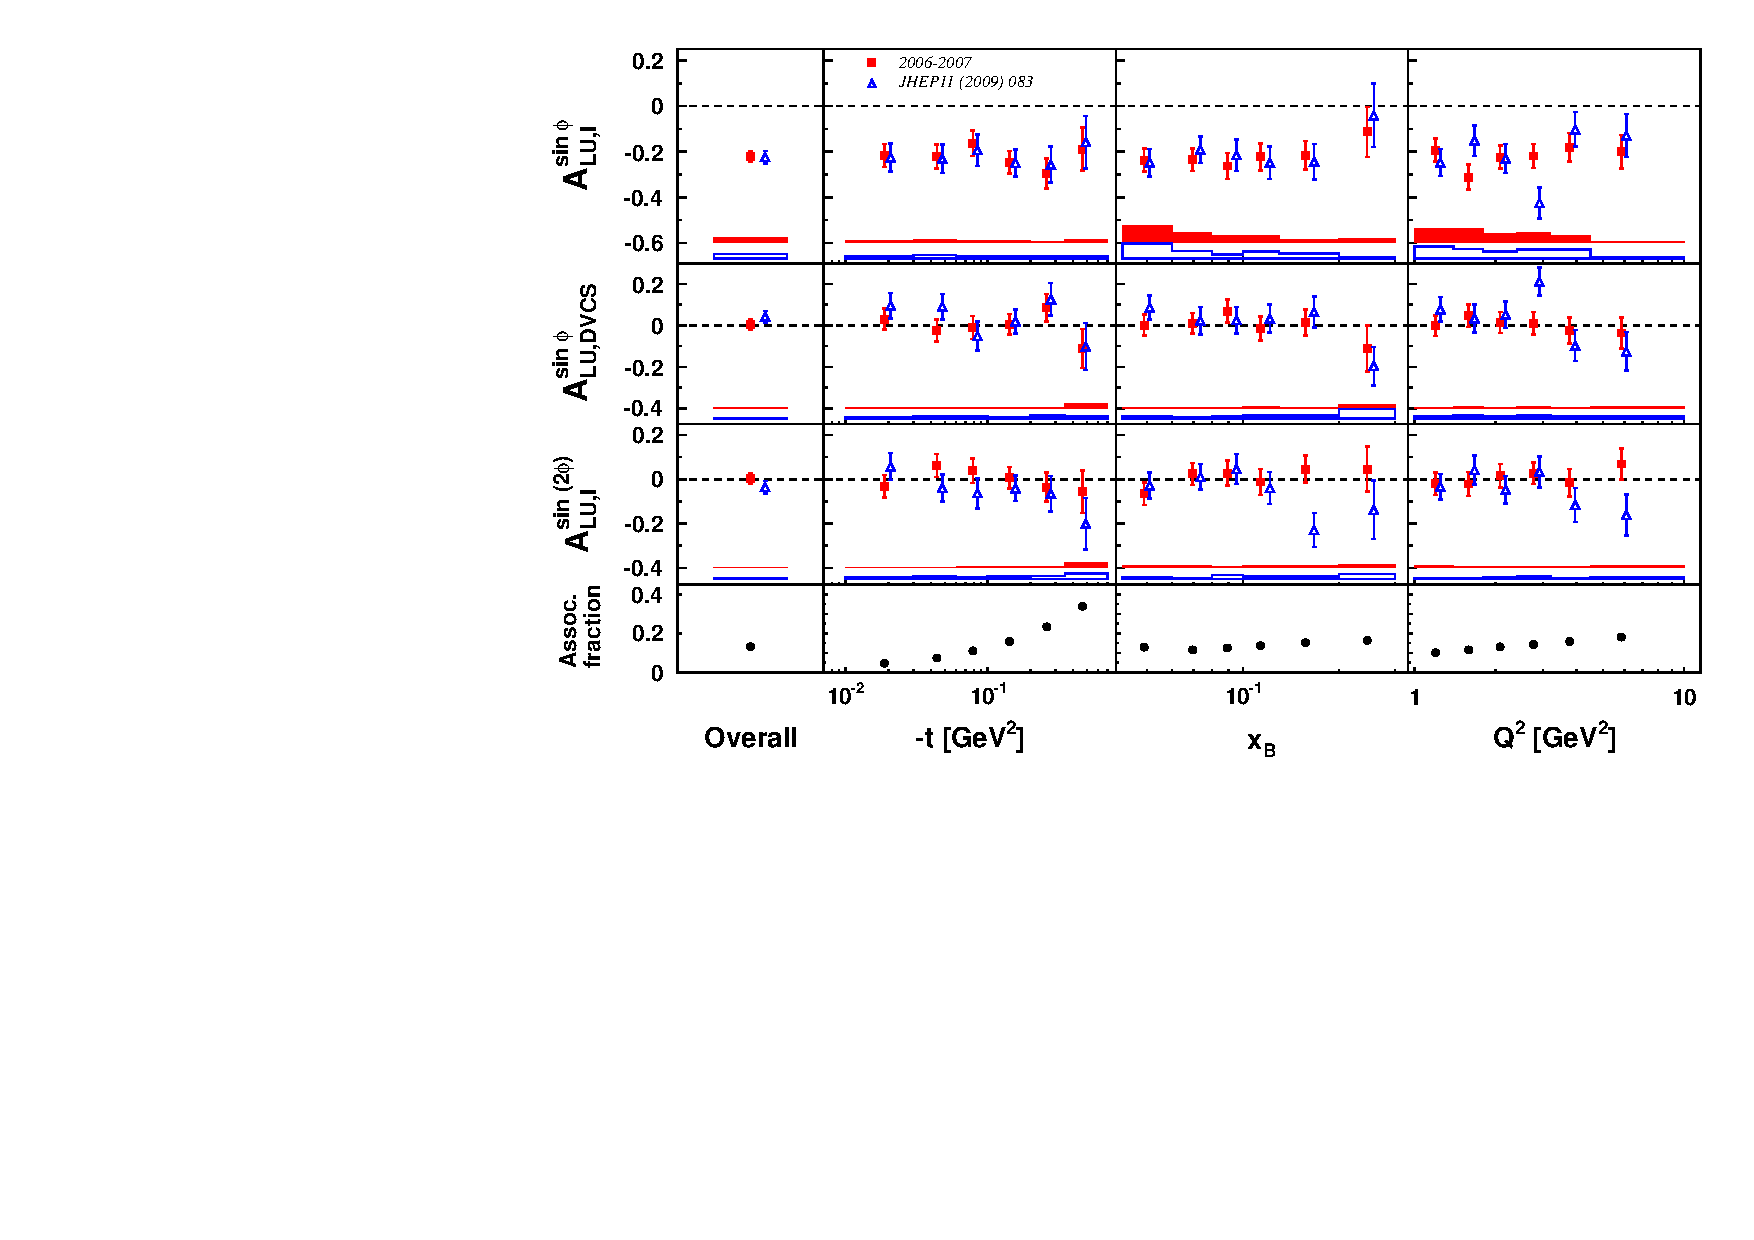
\includegraphics[width=15cm,keepaspectratio]{bsa_sep}
  \caption{Beam-helicity asymmetry amplitudes extracted separately from
the 1996-2005 (open triangles)~\cite{Air09} and 2006-2007 (filled squares)
hydrogen data. The error bars represent the statistical uncertainties. The error bands represent the systematic uncertainties.
An additional 2.8\,\% and 3.4\,\% scale uncertainty for the 1996-2005 and
2006-2007 data respectively is present in the amplitudes due to the uncertainty of
the beam polarisation measurement. The simulated fractional contribution from associated production to the yield in each kinematic bin is shown in the bottom row.}
 \label{release_bsa_0607}
\end{center}
 \end{figure}

A statistical test (Student's t-test) was applied in order to check for possible incompatibility between the asymmetry amplitudes extracted from the two data sets. Only the statistical uncertainties were employed in this test as the largest contributions to the systematic uncertainties, i.e. effects from detector resolution, acceptance, misalignment and smearing, are largely correlated. This test revealed no significant evidence for incompatibility between the data sets. The beam-helicity and beam-charge asymmetry amplitudes can therefore be extracted from the entire hydrogen data set recorded during the entire experimental operation of H{\sc ermes}.
\begin{figure}
\begin{center}
 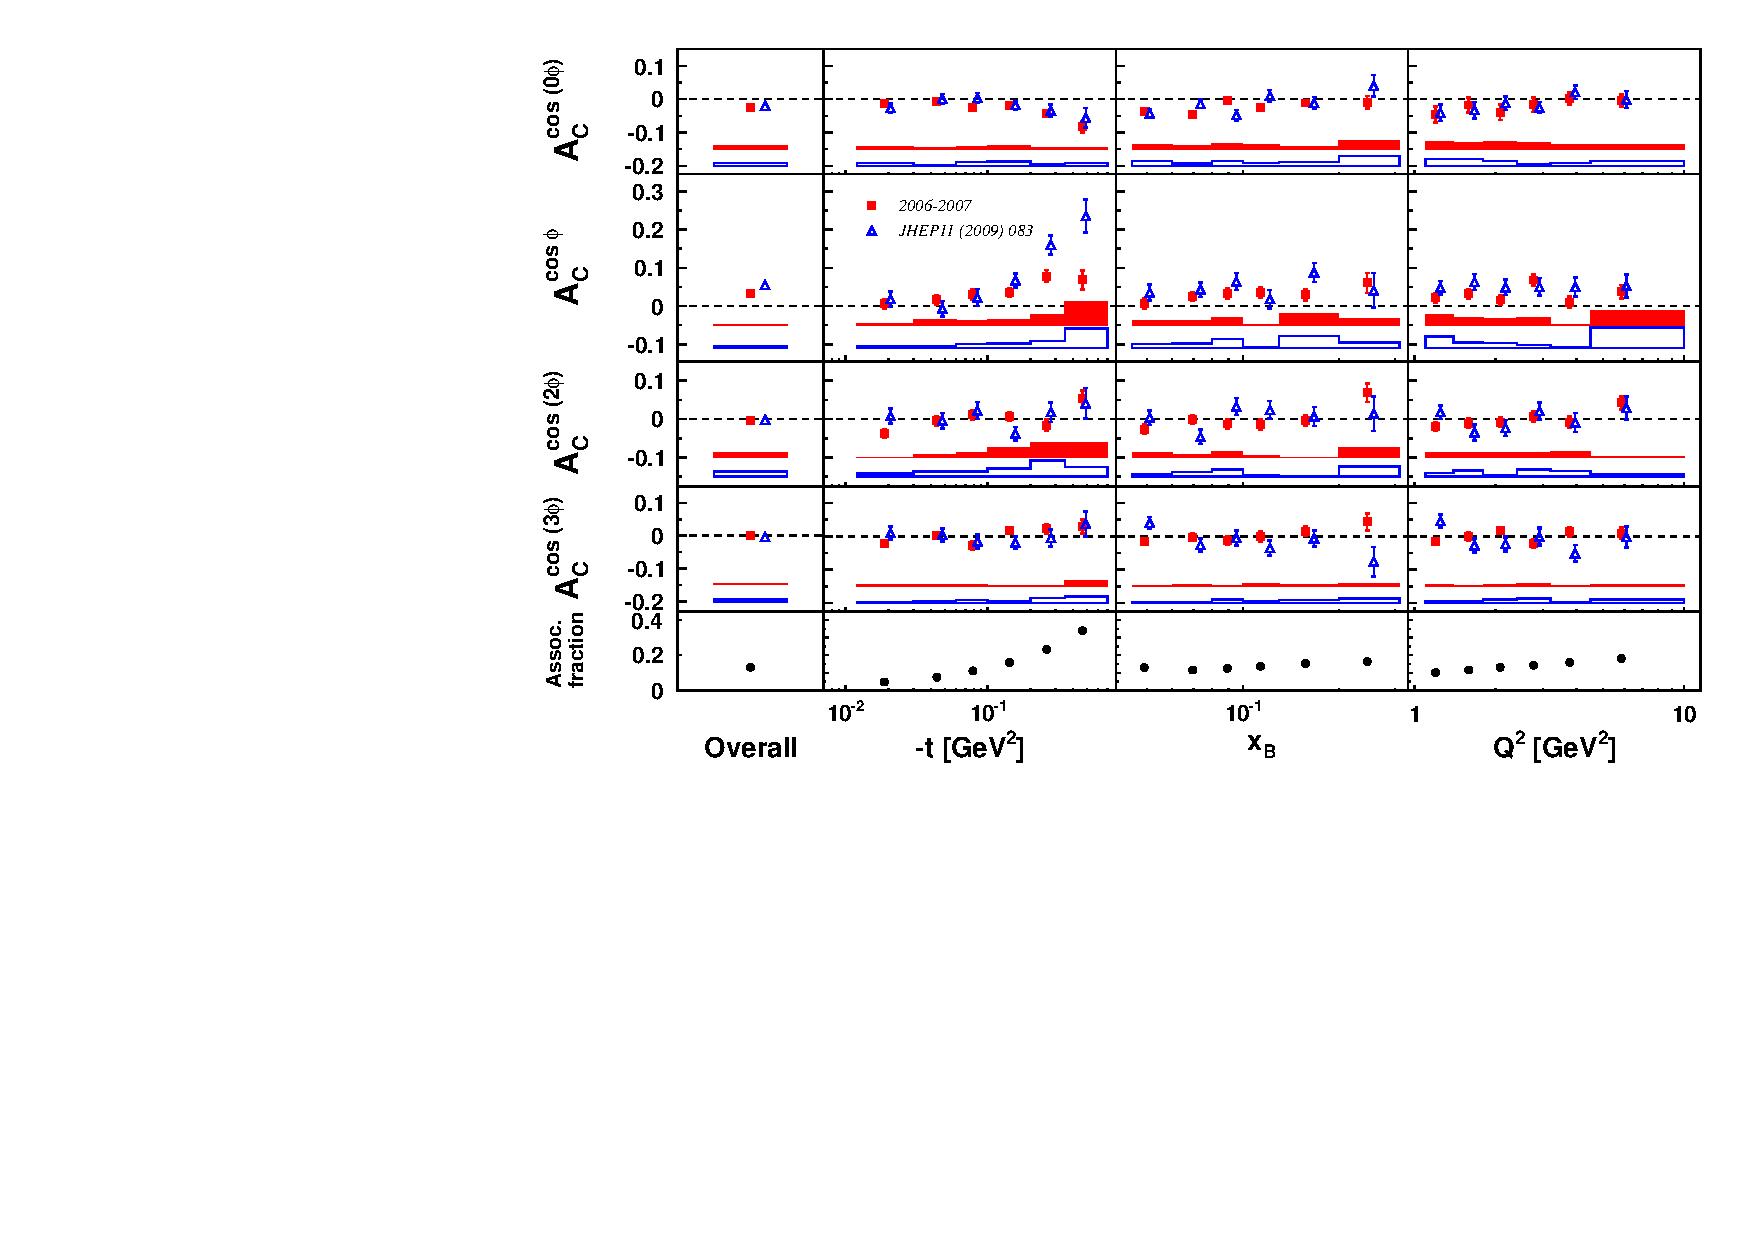
\includegraphics[width=15cm,keepaspectratio]{bca_sep}
  \caption{Beam-charge asymmetry amplitudes extracted separately from the 1996-2005 (open triangles)~\cite{Air09} and 2006-2007 (filled squares) hydrogen data.
The error bars represent the statistical uncertainties. The error bands represent the systematic uncertainties. The simulated fractional contribution from associated production to the yield in each kinematic bin is shown in the bottom row.}
 \label{release_bca_0607}
\end{center}
 \end{figure}

\begin{figure}
 \begin{center}
 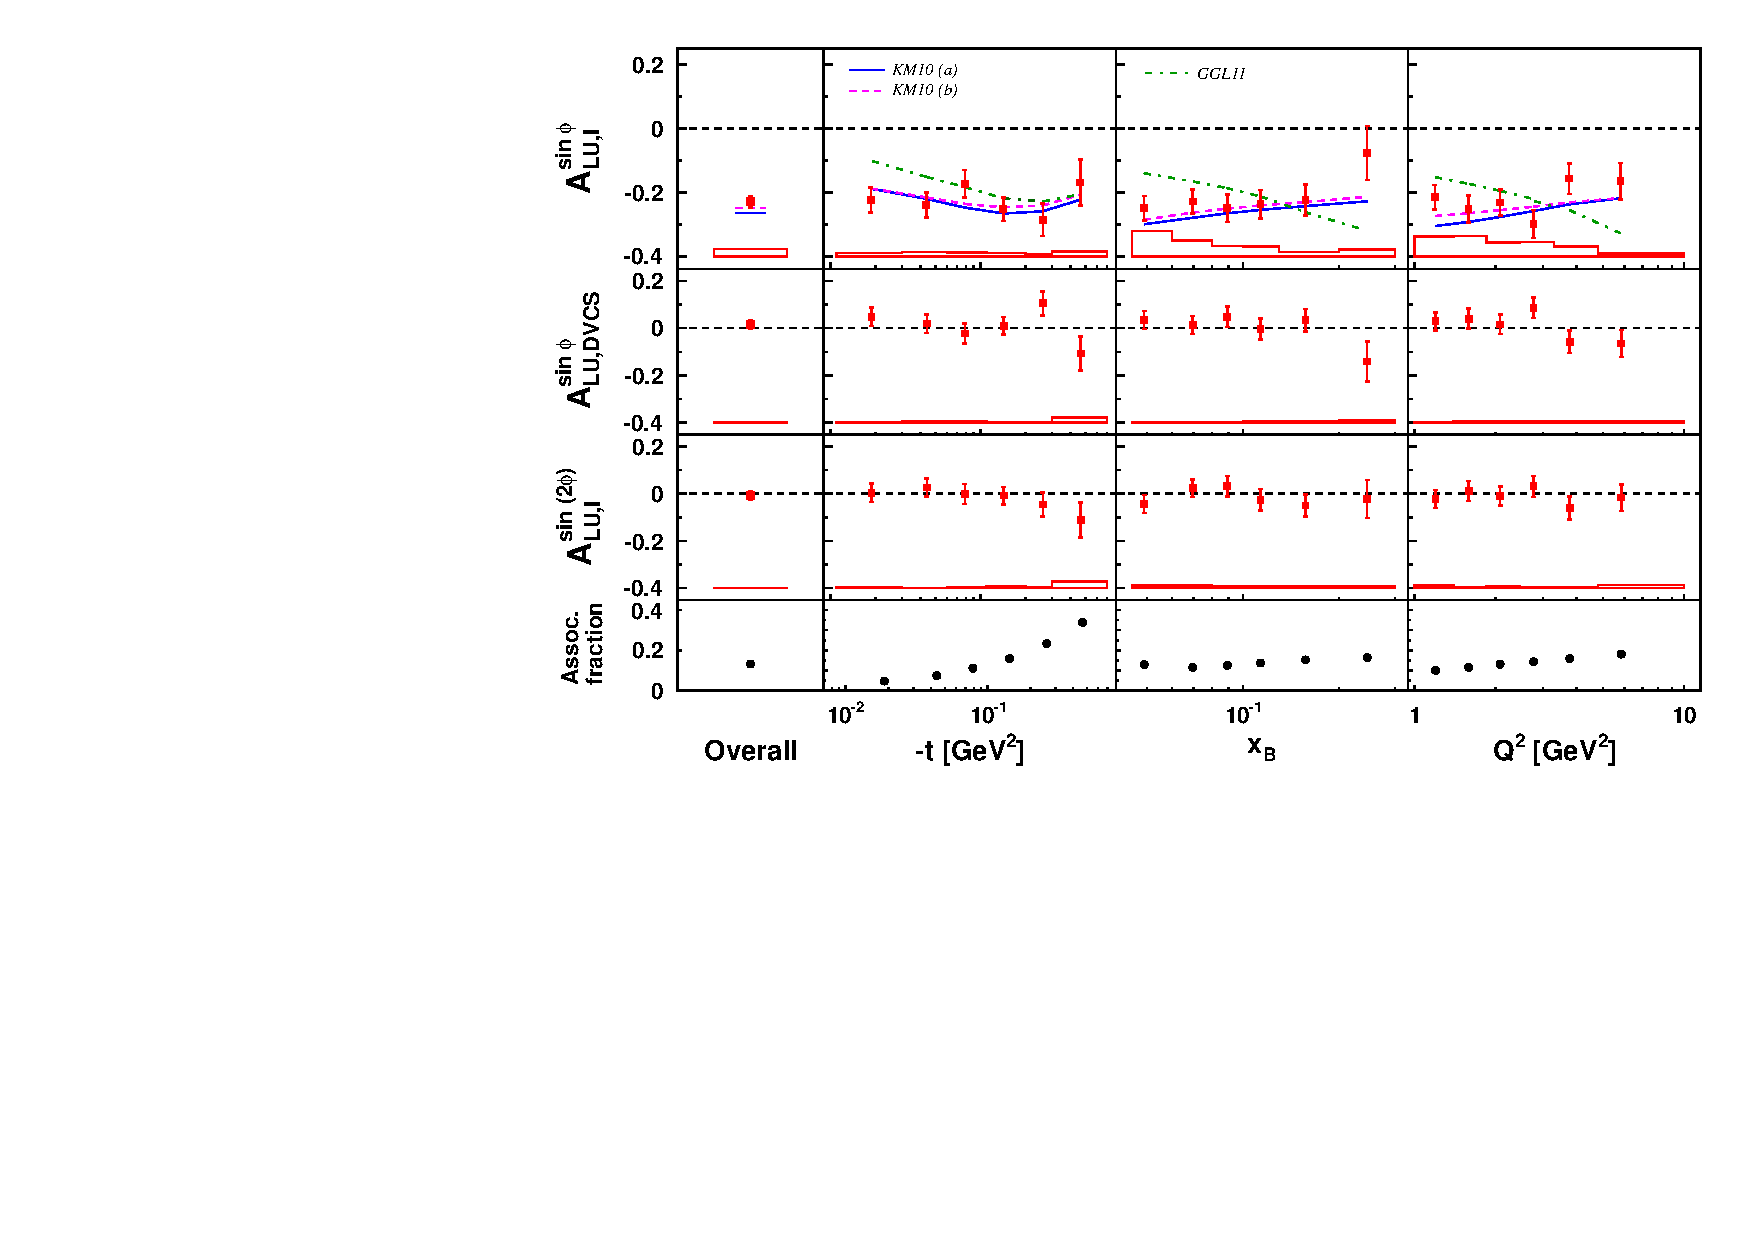
\includegraphics[width=15cm]{bsa_comb}
  \caption{The $A_{\textrm{LU,I}}^{\sin\phi}$, $A_{\textrm{LU,DVCS}}^{\sin\phi}$ and
$A_{\textrm{LU,I}}^{\sin(2\phi)}$ beam-helicity asymmetry amplitudes extracted from all the hydrogen data recorded at H{\sc ermes}
from 1996 until 2007. The error bars (bands) represent the statistical
(systematic) uncertainties. An additional 3.2\,\% scale uncertainty is present in the amplitudes due to the uncertainty of
the beam polarisation measurement. Solid and dashed lines (KM10) show model calculations from~\cite{Kum09}; calculations from Ref.~\cite{Liu11} are shown as dashed-dotted lines (GGL11). See text for details. The simulated fractional contribution from associated production to the yield in each kinematic bin is shown in the bottom row.}
  \label{bsa_xbjrange}
 \end{center}
\end{figure}

\begin{figure}
  \begin{center}
    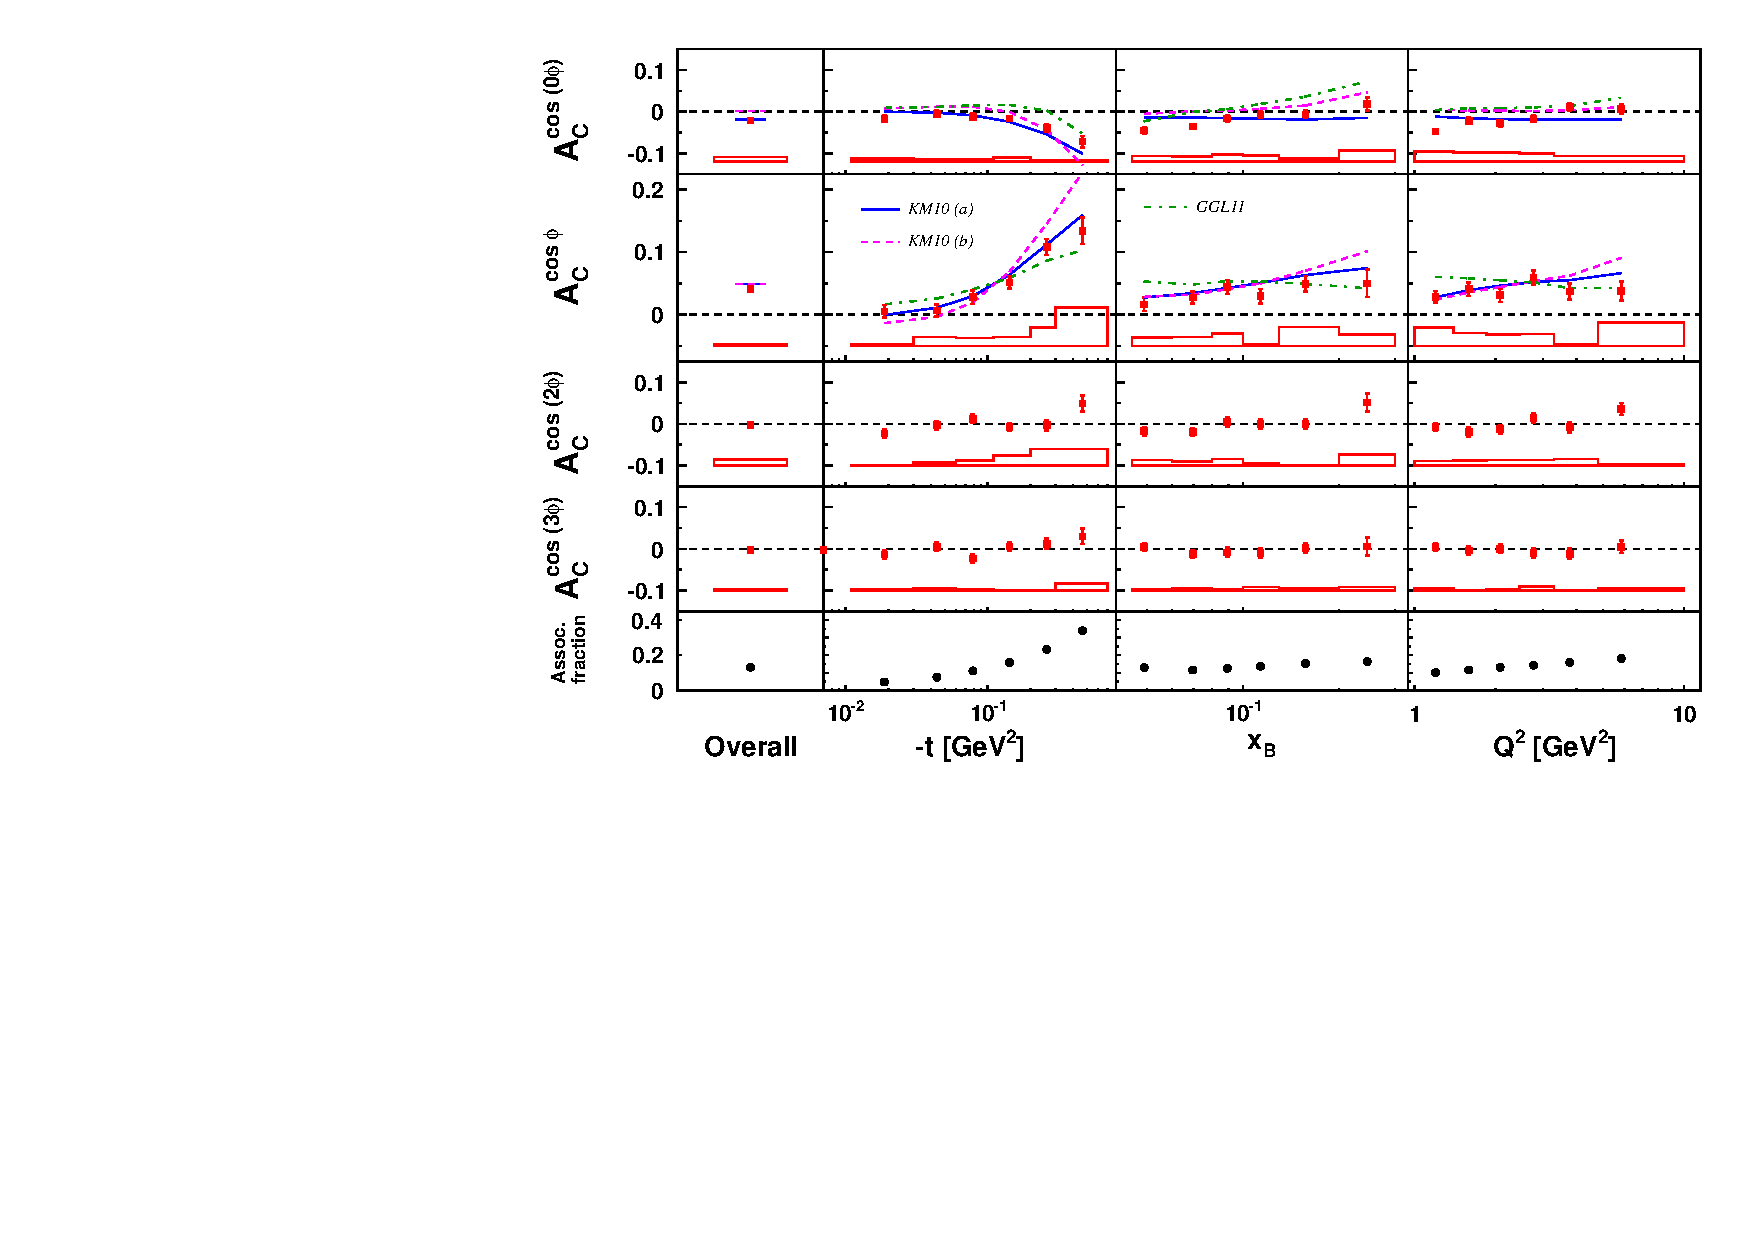
\includegraphics[width=15cm]{bca_comb}
    \caption{The $A_{\textrm{C}}^{\cos(0\phi)}$, $A_{\textrm{C}}^{\cos\phi}$, $A_{\textrm{C}}^{\cos(2\phi)}$ and $A_{\textrm{C}}^{\cos(3\phi)}$ beam-charge asymmetry amplitudes extracted from all the hydrogen data recorded at H{\sc ermes} from 1996 until 2007. The error bars (bands) represent the statistical (systematic) uncertainties.  Theoretical calculations from the model described in Ref. \cite{Kum09} are shown as solid and dashed lines (KM10); calculations from Ref.~\cite{Liu11} are shown as dashed-dotted lines (GGL11). See text for details. The simulated fractional contribution from associated production to the yield in each kinematic bin is shown in the bottom row.}
  \label{bca_xbjrange}
 \end{center}
\end{figure}

\begin{figure}
 \begin{center}
 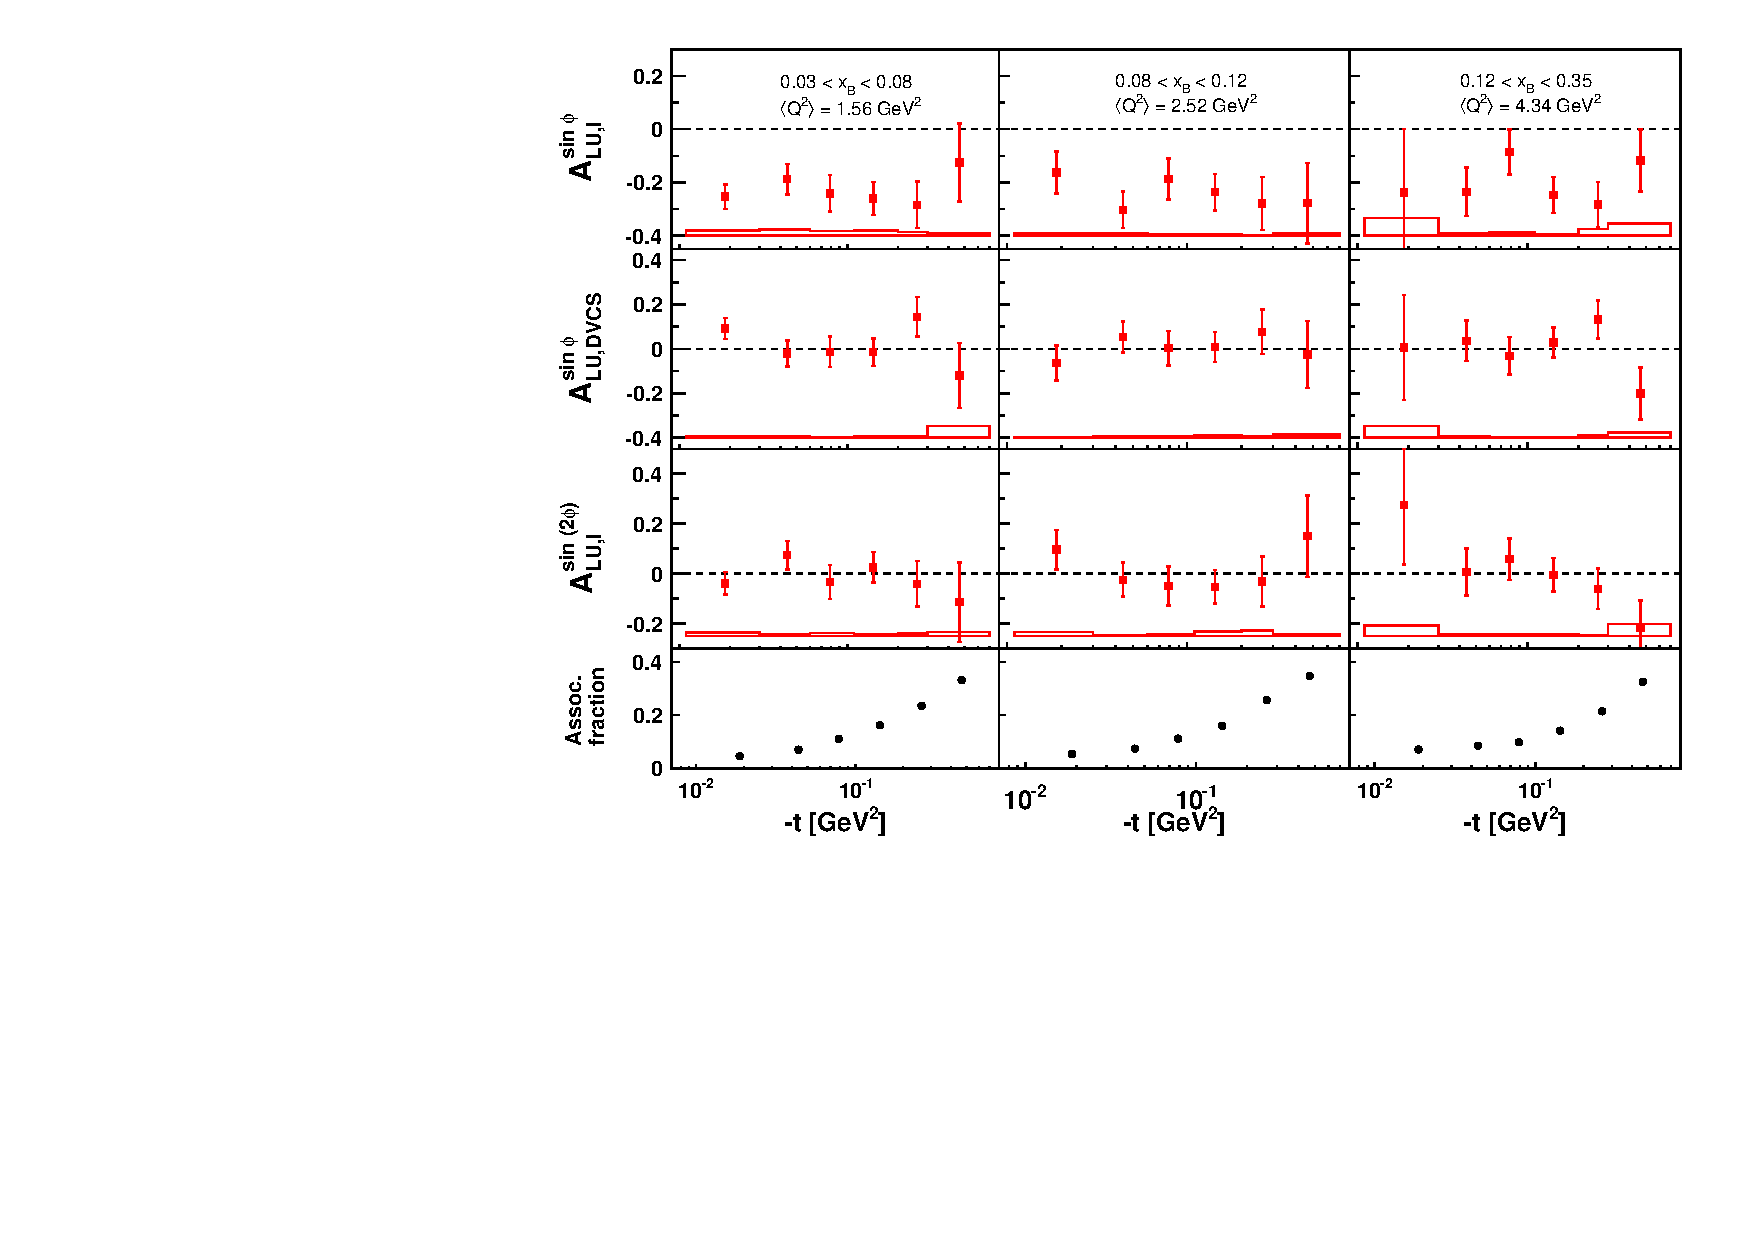
\includegraphics[width=15cm]{bsa_2D}
  \caption{The $A_{\textrm{LU,I}}^{\sin\phi}$, $A_{\textrm{LU,DVCS}}^{\sin\phi}$ and
$A_{\textrm{LU,I}}^{\sin(2\phi)}$ beam-helicity asymmetry amplitudes extracted from all the hydrogen data recorded at H{\sc ermes} from 1996 until 2007 as a function of $-t$ for three different $x_{\textrm{B}}$ ranges. The error bars (bands) represent the statistical (systematic) uncertainties. An additional 3.2\,\% scale uncertainty is present in the amplitudes due to the uncertainty of the beam polarisation measurement. The simulated fractional contribution from associated production to the yield in each kinematic bin is shown in the bottom row.}
  \label{bsa_xbjrange2}
 \end{center}
\end{figure}

\begin{figure}
  \begin{center}
    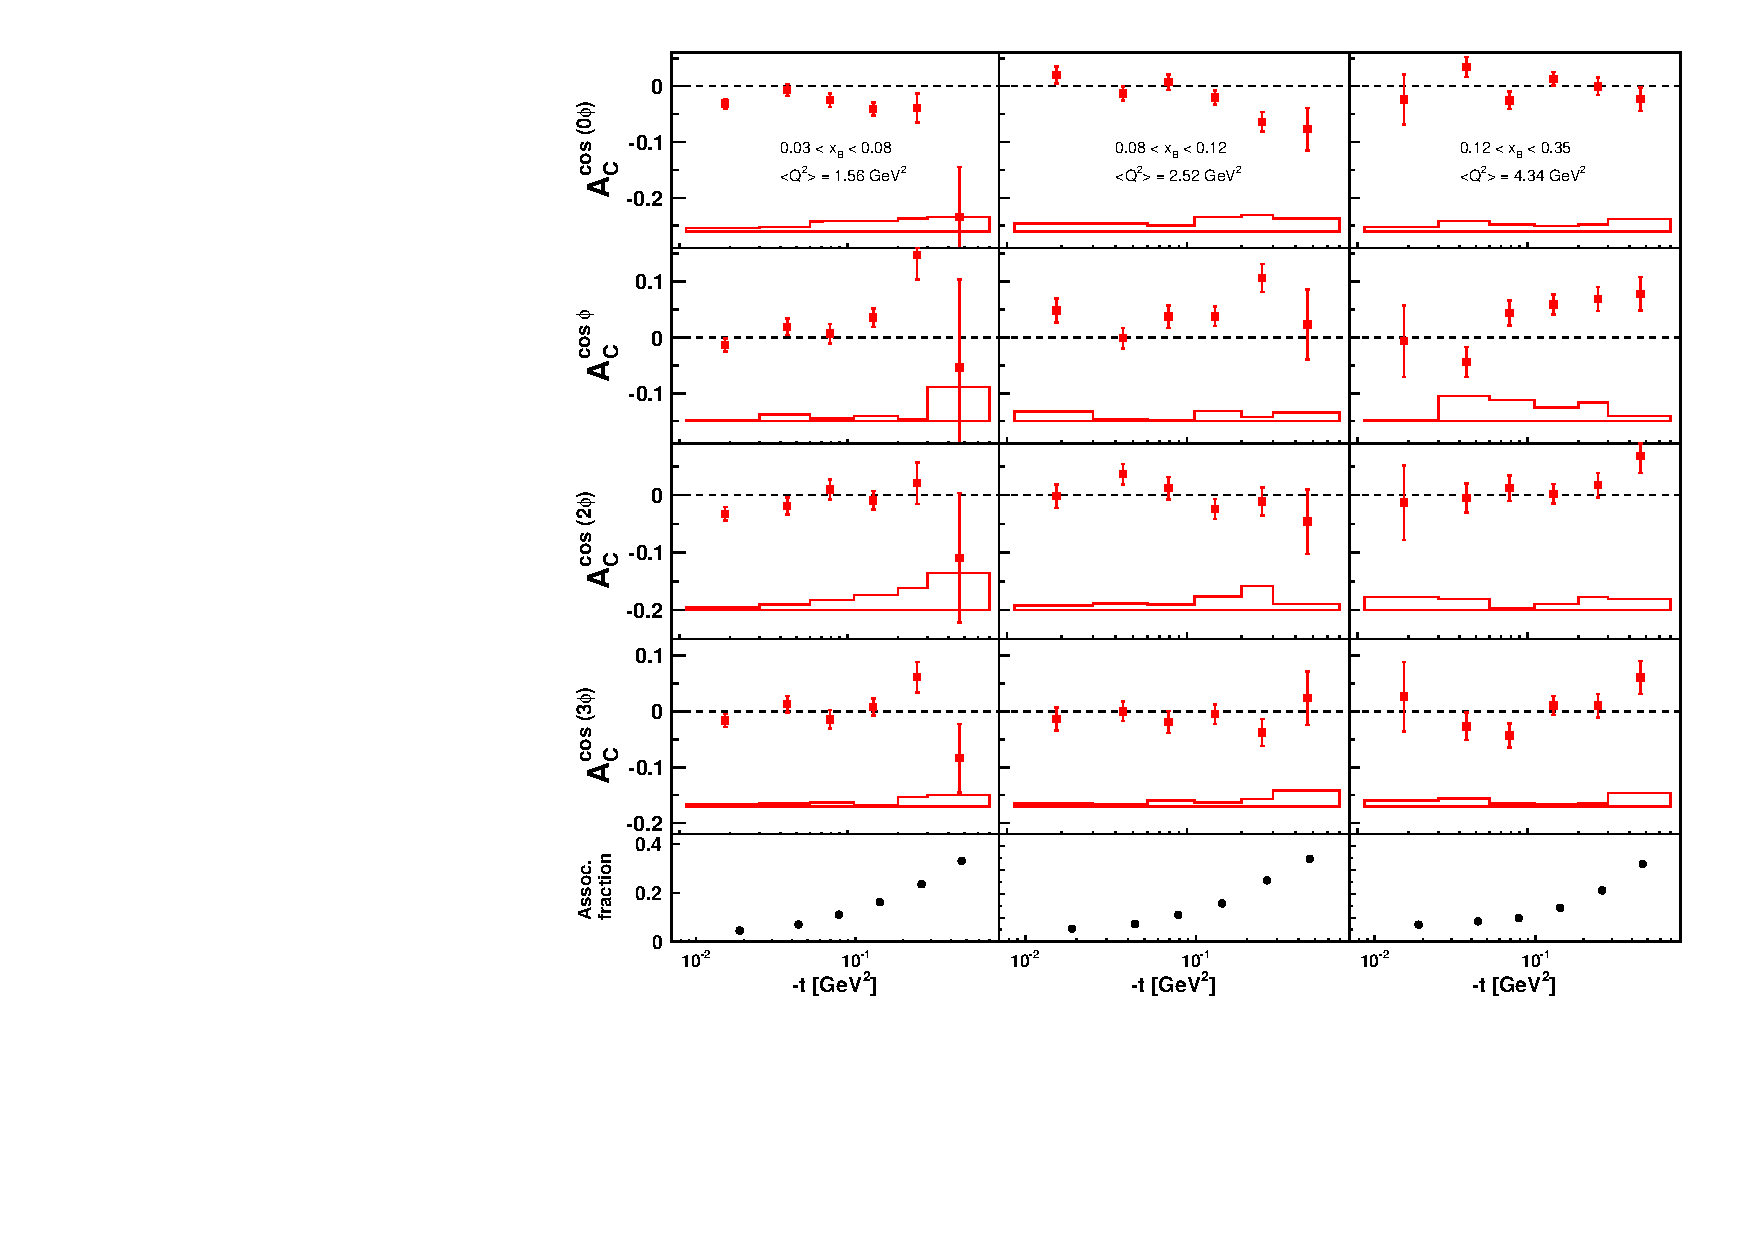
\includegraphics[width=15cm]{bca_2D}
    \caption{The $A_{\textrm{C}}^{\cos(0\phi)}$, $A_{\textrm{C}}^{\cos\phi}$, $A_{\textrm{C}}^{\cos(2\phi)}$ and $A_{\textrm{C}}^{\cos(3\phi)}$ beam-charge asymmetry amplitudes extracted from all the hydrogen data recorded at H{\sc ermes} from 1996 until 2007 as a function of $-t$ for three different $x_{\textrm{B}}$ ranges. The error bars (bands) represent the statistical (systematic) uncertainties. The simulated fractional contribution from associated production to the yield in each kinematic bin is shown in the bottom row.}
  \label{bca_xbjrange2}
 \end{center}
\end{figure}

The results of the beam-helicity and beam-charge asymmetry amplitudes extracted from the complete 1996-2007 hydrogen sample are shown in figures~\ref{bsa_xbjrange} and \ref{bca_xbjrange}. The number of analysable events available from the 2006-2007 data set (70352) is approximately three times greater than the number of events recorded in the 1996-2005 sample (24817). The  asymmetry amplitudes extracted from the complete 1996-2007 data set thus resemble the 2006-2007 result. This resemblance is not so evident for the beam-helicity asymmetry amplitudes as it is for the beam-charge asymmetry amplitudes, because the beam polarisation was lower in 2006 and 2007 than in 1996-2005 and thus the 2006-2007 data has a lower weighting in the combined fit. The major contributions to the systematic error bands associated with the asymmetry amplitudes extracted from the combined data set were determined using Monte Carlo simulations as explained in section~4, i.e. contributions from acceptance, smearing, finite bin widths and misalignment. The background in the \red{combined} data sample is estimated using the method from refs.~\cite{Air08,Zei09, Bur10}. The uncertainty contributions due to the observed shifts in the missing-mass distributions for the combined data sets were calculated using the procedure described in section~4 and the results were averaged. The total systematic uncertainties for the combined results are \red{obtained by adding these} three independent contributions in quadrature.
The first and second harmonics of $\mathcal{A}_{\textrm{LU,I}}$, which are
sensitive to the interference term in the scattering amplitude, are shown in the first and third rows of figure~\ref{bsa_xbjrange}. The leading-twist amplitude $A_{\textrm{LU,I}}^{\sin\phi}$ has the largest magnitude of any of the amplitudes when extracted in a single bin from the entire data set. This amplitude shows no strong dependence on $-t$, $x_{\textrm{B}}$ or $Q^{2}$, implying a strong dependence at smaller values of $-t$ as the amplitude must approach zero as $-t$ approaches its minimum value because of the dependence of the amplitude on the factor $K$ defined in eq.~\ref{eq:K}. The $A_{\textrm{LU,I}}^{\sin\phi}$ amplitude is sensitive to the imaginary part of the CFF $\mathcal{H}$ and thereby can constrain GPD $\textit{H}$. The $A_{\textrm{LU,DVCS}}^{\sin\phi}$ asymmetry is shown in the second row of figure~\ref{bsa_xbjrange}. Both the $A_{\textrm{LU,DVCS}}^{\sin\phi}$ asymmetry amplitude and the $A_{\textrm{LU,I}}^{\sin(2\phi)}$ asymmetry amplitude are compatible with zero, and neither asymmetry amplitude shows any dependence on $-t$, $x_{\textrm{B}}$ or $Q^{2}$.

The $A_{\textrm{C}}^{\cos(n\phi)}$ amplitudes are shown in figure~\ref{bca_xbjrange}. The systematic uncertainties are estimated using the same procedure as was used to estimate those for the beam-helicity asymmetries. The leading twist $A_{\textrm{C}}^{\cos(0\phi)}$ and $A_{\textrm{C}}^{\cos\phi}$ amplitudes are both non-zero. There is an expected relationship between $A_{\textrm{C}}^{\cos(0\phi)}$ and $A_{\textrm{C}}^{\cos\phi}$ as they depend on the same $\mathcal{C}$-function. The kinematic suppression of $A_{\textrm{C}}^{\cos(0\phi)}$ with regard to $A_{\textrm{C}}^{\cos\phi}$ is approximately fulfilled. The measured amplitudes are found to diverge with opposite sign from zero at increasing values of $-t$ and they indicate a weak increase with $x_{\textrm{B}}$ and $Q^{2}$. The $A_{\textrm{C}}^{\cos(2\phi)}$ and $A_{\textrm{C}}^{\cos(3\phi)}$ amplitudes are both consistent with zero over the whole range in $-t$, $x_{\textrm{B}}$ and $Q^{2}$. The $A_{C}^{\cos(2\phi)}$ amplitude is related to twist-3 GPDs and $A_{\textrm{C}}^{\cos(3\phi)}$ relates to gluon helicity-flip GPDs. Both of these amplitudes are expected to be suppressed at H{\sc ermes} kinematic conditions compared to the leading twist amplitudes. 

The curves in  figures~\ref{bsa_xbjrange} and~\ref{bca_xbjrange} show the results of model calculations at the average value of the kinematic bins used for the data analysis. The solid and dashed curves show results of calculations from a global fit of GPDs to experimental data~\cite{Kum09} including information from H{\sc ermes} and Jefferson Lab., and the collider experiments at H{\sc era}. The basic model~\cite{Mue05,Kum07,Kum08} is a \red{flexible GPD representation that is based on both a Mellin-Barnes integral and dispersion integral representation with weakly entangled skewedness and $t$ dependences}. The solid curves represent the model fit without data from experiments \cite{Cam06} at Hall A of Jefferson Lab.; the model fit represented by the dashed curves includes 1these data. Both fits include the 1996-2005 H{\sc ermes} data. The model incorporates only twist-2 GPDs and so can provide results only for the $A_{\textrm{LU,I}}^{\sin\phi}$, $A_{\textrm{C}}^{\cos(0\phi)}$ and $A_{\textrm{C}}^{\cos\phi}$ asymmetry amplitudes. All of the relevant amplitudes reported here are well described by the model.

The dash-dotted curves in figures~\ref{bsa_xbjrange} and~\ref{bca_xbjrange} show the result of calculations from a fit based on a quark-diquark model with a Regge-inspired term that is included in order to describe accurately parton distribution functions at low $x$ values~\cite{Liu11}. The ``Regge'' term is extended to include contributions that determine the $t$-dependence of the corresponding GPD. The model incorporates fits to global deep-inelastic and elastic scattering data (to account for the $\xi$-independent limits and moments of the underlying GPDs) and DVCS data from Jefferson Lab. (to describe the skewness dependence). The model describes the $t$-projections of the $A^{\sin\phi}_{\textrm{LU}}$ amplitude reported here well, but the projections in the other kinematic variables are not as well described. The model describes the trends of the $A_{\textrm{C}}^{\cos(0\phi)}$ and $A_{\textrm{C}}^{\cos\phi}$ asymmetry amplitudes well.

In order to provide more detailed information that can be used in future fits, in particular for the determination of the entanglement of the skewness and $-t$ dependences of GPDs, the amplitudes already presented in figures~\ref{bsa_xbjrange} and~\ref{bca_xbjrange} are shown as a function of $-t$ for three different ranges of $x_{\textrm{B}}$ in figures~\ref{bsa_xbjrange2} and~\ref{bca_xbjrange2}. These figures represent the kinematic dependences of the amplitudes in a less-correlated manner than the one\red{-}dimensional projections: within experimental uncertainty, there is no evidence of a correlation between the $-t$ and $x_{\textrm{B}}$ dependence\red{s} for any of the amplitudes. The results from this paper will be made available in the Durham Database. The results will also be made available in the same 4 bin format as used in previous analyses at H{\sc ermes}~\cite{Air08,Air09,Air10b}.
